\chapter{Validation}

\section{Introduction}
After building our model inside the \textbf{OMNeT++} we can proceed with the simulation in order to analyze the quantities wich we are interested. First of all we will simulate the model in very simple cases in order to be sure it reproduces the system's behavior correctly. We decided to validate our model by \textit{removing randomness}. This choice allows us to do some easy computation by hand and to verify if the result of simulation is consistent with them. Our model will be considered a good replica of the system if it will pass all the \textit{validation tests}. During the validation we will use the first scheduler: \textbf{Round-Robin Frame Fill} because it generates simulation which are easier to analyze and to compare with analitical results.

\section{1\textsuperscript{st} test: fixed CQI, fixed \(\lambda\) rate, fixed packet size, 1 user}
In this test we just one \texttt{Mobile Station} connected to the antenna wich always generates the same CQI for each timeslot. Inside the \texttt{Web Server} the \(\lambda\) rate is fixed and also the packet size. This is a very simple system with deterministic arrivals and deterministic service demand. We can compute the traffic that \texttt{Web Server} sends to the antenna as \[ th\textsubscript{in} = \frac{packetsize \times 8}{1/(1000\lambda)} \lbrack bps \rbrack \] 
If the system is in a stable state the output throughput and the input throughput must be equal. The maximum output throughput is the one we have by setting all parameters to maximum values. \[ th\textsubscript{max} = \frac{\#RB \times RBsize\textsubscript{max} \times 8}{T\textsubscript{slot}} = \frac{25 \times 93 \times 8}{0.001} = 18.6 \textnormal{ Mbps} \] We can derive very easily the \(\lambda\textsubscript{max}\) rate wich produces the max throughput allowed by antenna. \[\lambda\textsubscript{max} = \frac{\#RB \times RBsize\textsubscript{max}}{1000 \times T\textsubscript{slot} \times packetsize\textsubscript{max}} = \frac{25 \times 93}{1000 \times 0.001 \times 75} = 31 \textnormal{ ms\textsuperscript{-1}} \] For \( 0<\lambda<\lambda\textsubscript{max} \) the system is a stable state and so \(th\textsubscript{in} = th\textsubscript{out}\). For higher \(\lambda\) the FIFOQueue grows indefinitely because the frame is not able to carry as much data in a time slot.

Let's consider all the simulations with the following parameters:
\begin{itemize}
	\item \(\lambda \in \{1,2,\ldots,32\}\)
	\item \(packetsize=75\)
	\item \(CQI=15\)
\end{itemize}
  We can se in the graph a linear behavior regarding the throughput until the system is not saturated. Note that the response time for each packet is zero since there is no queueing until \(\lambda < \lambda\textsubscript{max}\) and grows indefinitely when the system saturates. This is not surprising since \(th\textsubscript{in} \propto \lambda\) when \(\lambda < \lambda\textsubscript{max}\) and packet's size is fixed.
\begin{figure}[H]
  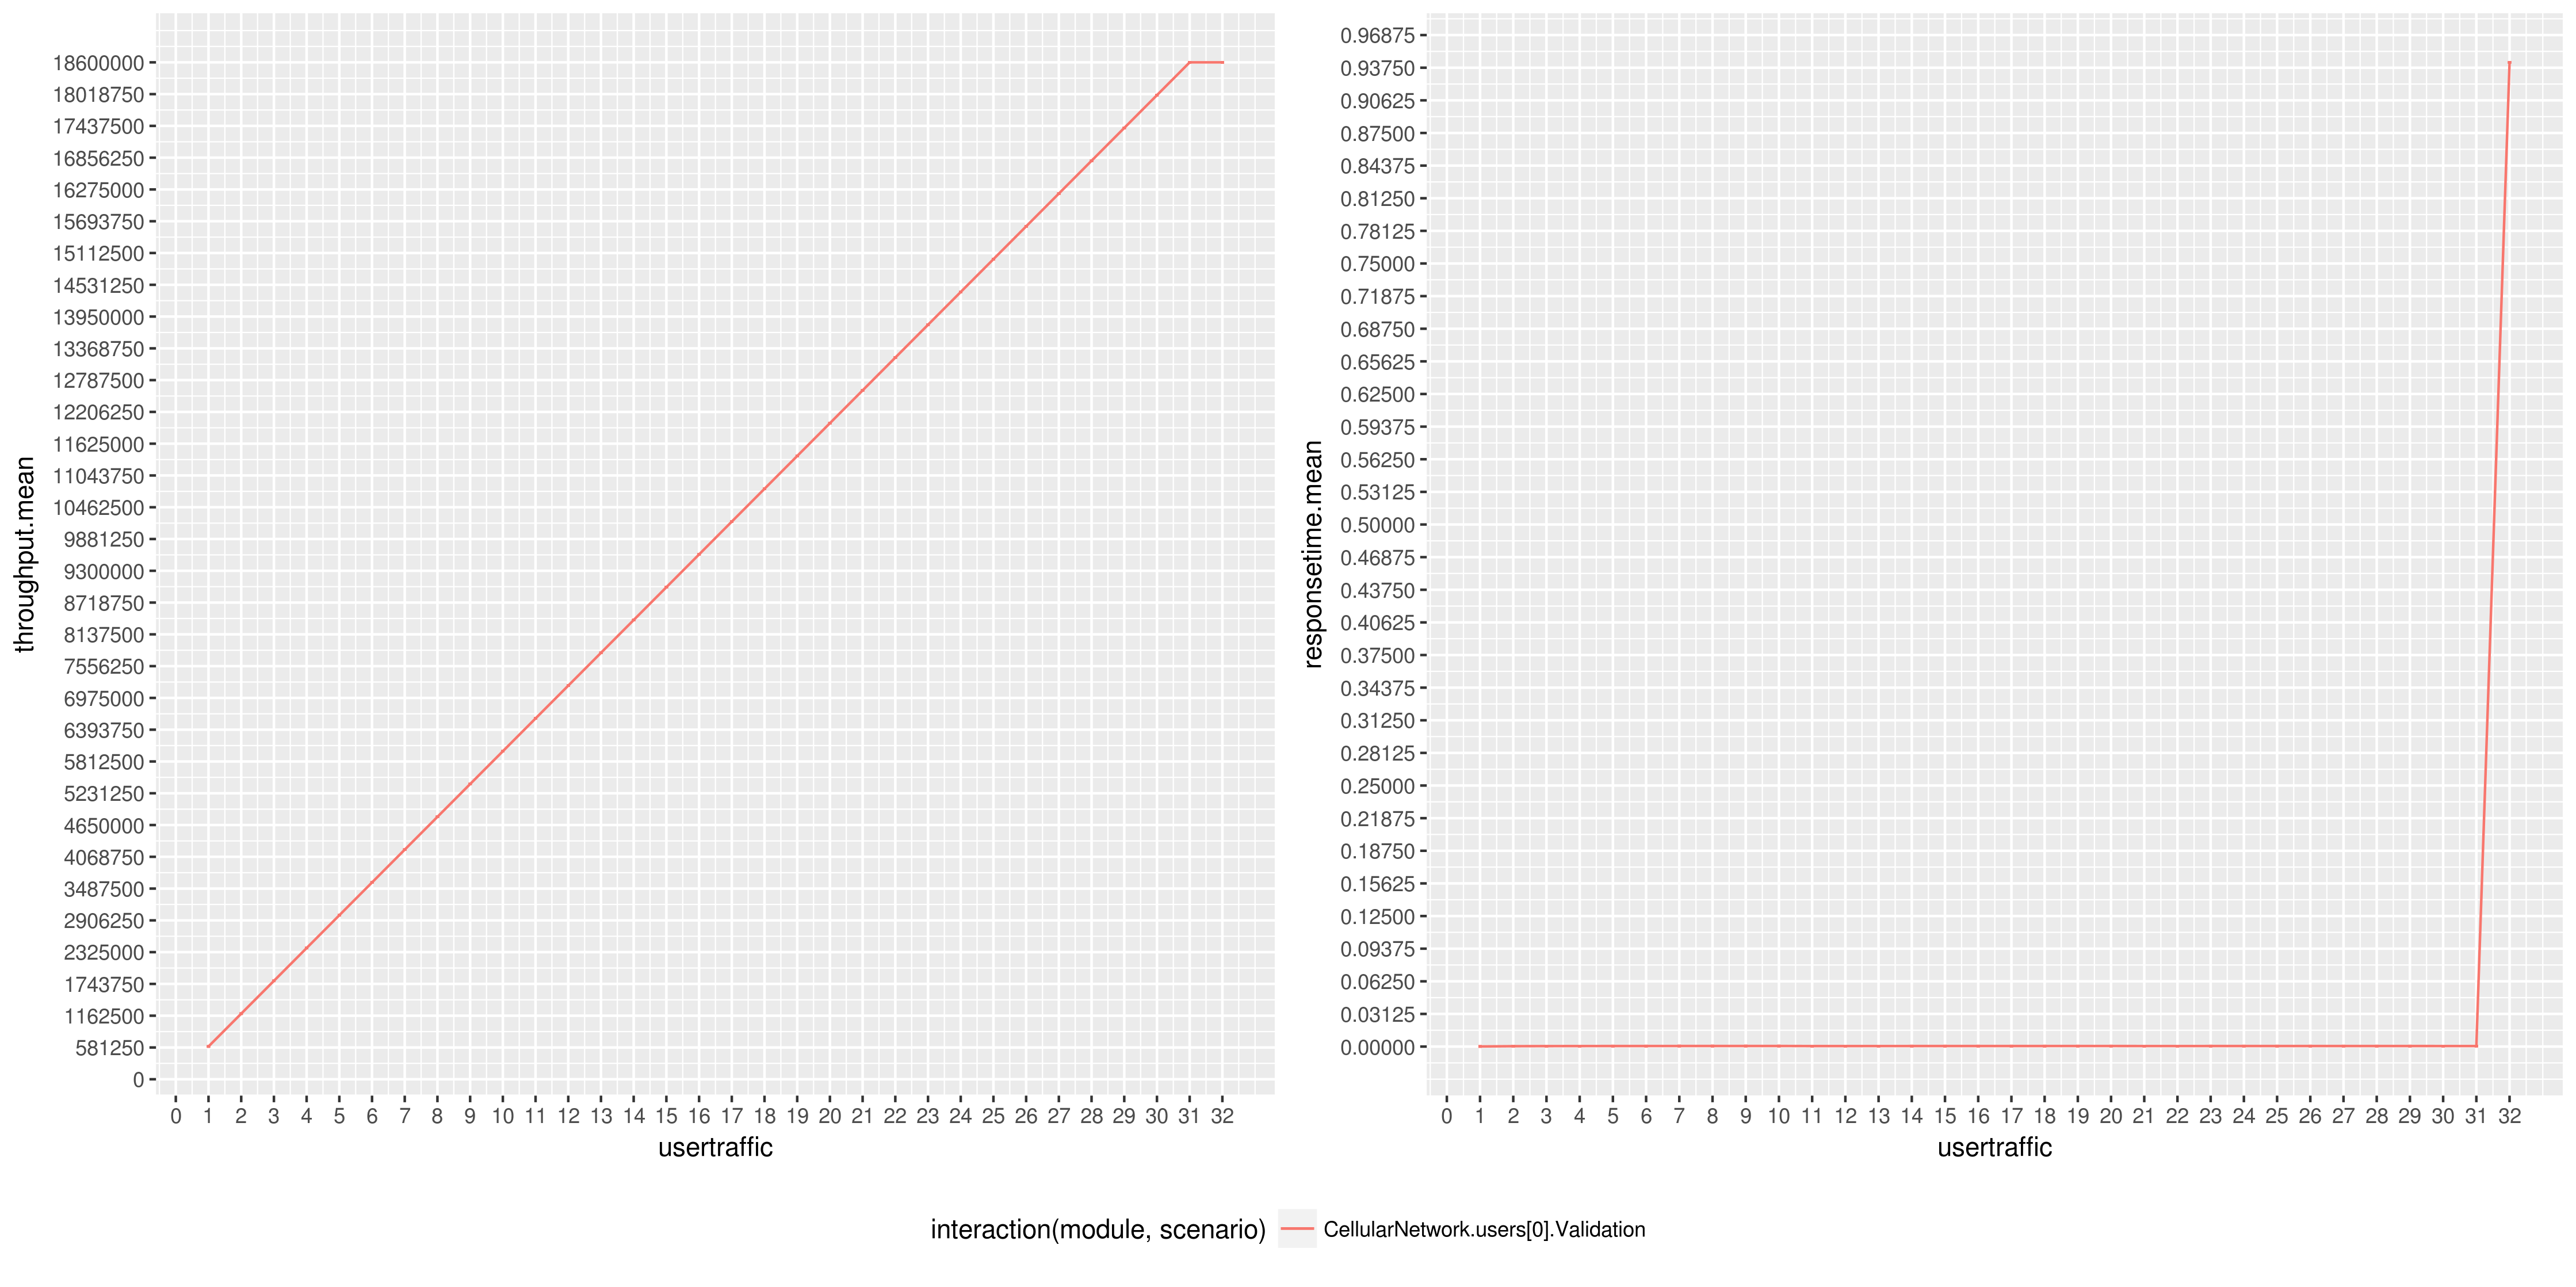
\includegraphics[width=1\textwidth]{images/plotvalidation}
  \caption{1st validation scenario: throughput, response time}
  \label{fig:1st validation scenario: throughput, response time}
\end{figure}

\section{2\textsuperscript{nd} test: fixed CQI, fixed \(\lambda\) rate, fixed packet size, 2 users}
In this test there are two \texttt{Mobile Stations} connected to antenna. As in the previous scenario all parameters are fixed. We have two indipendent flow of data from \texttt{Web Servers} to \texttt{Antenna} so the input throughtput could by computed as
\[ th\textsubscript{in} = \frac{packetsize\textsubscript{0} \times 8}{1/(1000\lambda\textsubscript{0})} + \frac{packetsize\textsubscript{1} \times 8}{1/(1000\lambda\textsubscript{1})}\]
For these simulation we have chosen the following parameters:
\begin{itemize}
	\item \(packetsize_{0} = packetsize_{1} = 40\)
	\item \(CQI_{0} = 6\)
	\item \(CQI_{1} = 15\)
	\item \(\lambda = \lambda_{0} = \lambda_{1}\) and \(\lambda \in \{1,2,\ldots,32\}\)
\end{itemize}
We can compute the max \textit{slotted thorughput} for both users.
\begin{align}
	slotth^{0}_{out} &= \frac{\#RB \times RBsize_{0} \times 8 }{T_s} = \frac{25 \times 20 \times 8}{0.001} = 4 \textnormal{ Mbps}\nonumber \\ 
	slotth^{1}_{out} &= \frac{\#RB \times RBsize_{1} \times 8 }{T_s} = \frac{25 \times 93 \times 8}{0.001} = 18.6 \textnormal{ Mbps} \nonumber
\end{align} 
At full load we expect that users compete to fill the frame. If the scheduler were fair, at full load, the average throughput would be \(th^{i}_{out} = (slotth^{i}_{out})/2\) since there are 2 users and the scheduler follow a round robin scheme, which is fair in principle. 
\begin{figure}[H]
  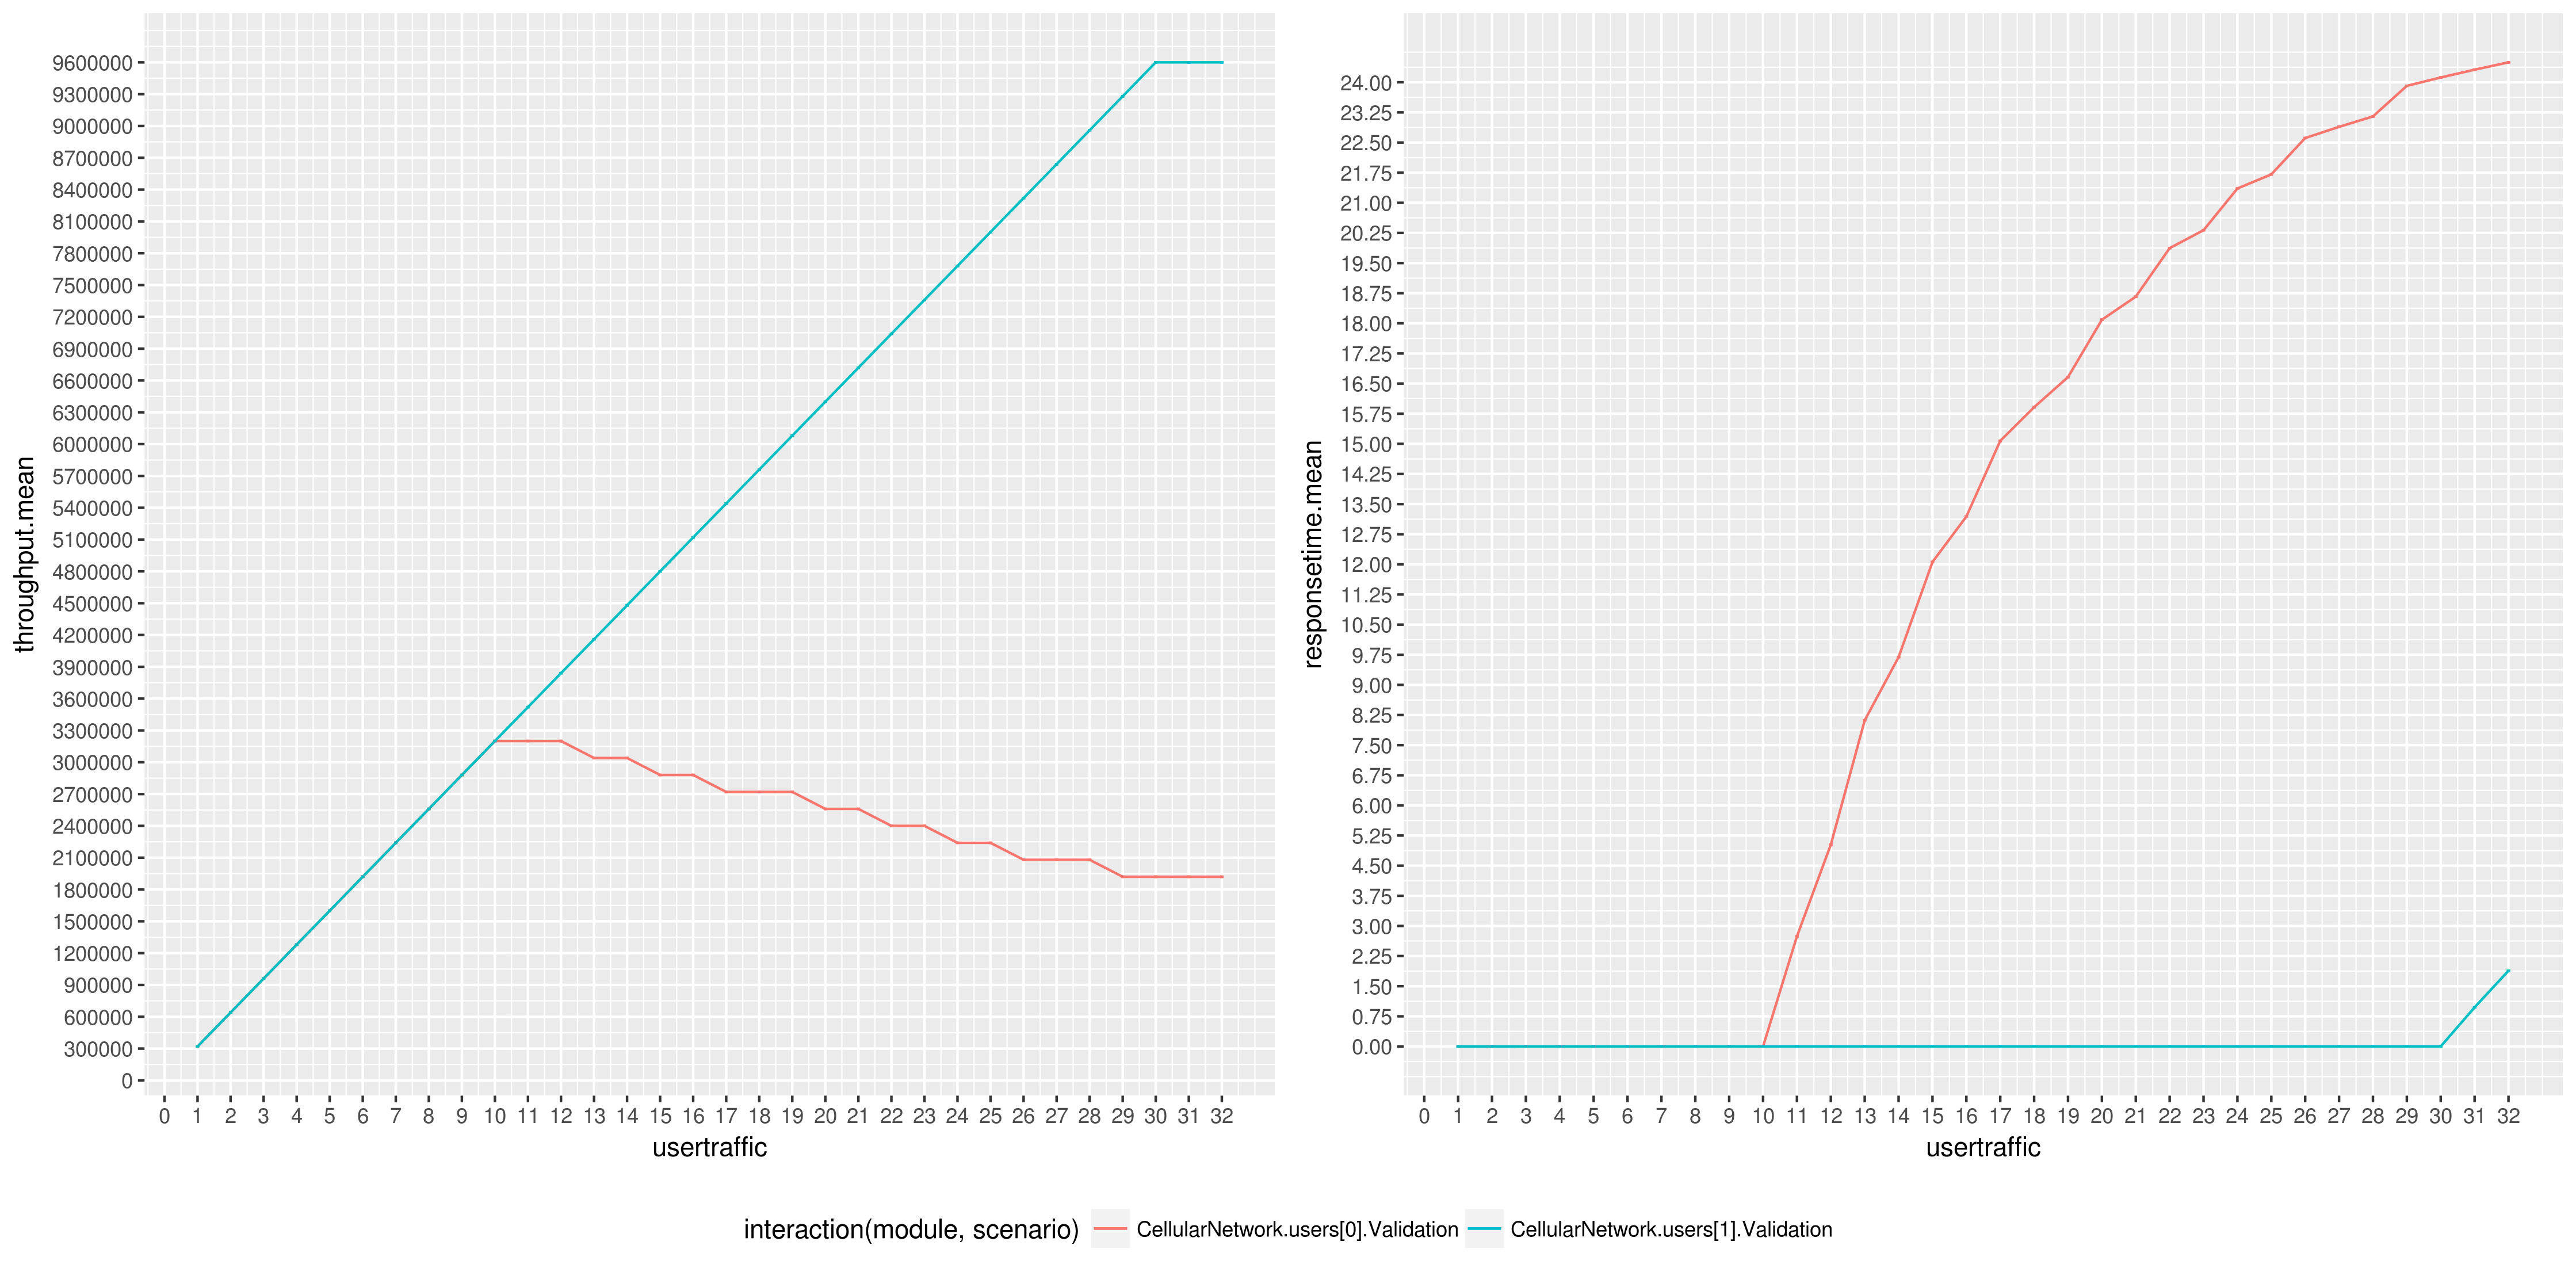
\includegraphics[width=1\textwidth]{images/plotvalidation2}
  \caption{2nd validation scenario: throughput, response time}
  \label{fig:2nd validation scenario: throughput, response time}
\end{figure}
We see in the graph that throghput grows linear ad is equal for both users when \(1 \leq \lambda \leq 10 \). For \(\lambda > 10 \) the \texttt{Mobile User[0]} saturates, conversely \texttt{Mobile User[1]} continues to increase its throughput until it reaches saturation at \(\lambda = 30\).
When \(\lambda = 10 \) the input flow is \(th_{in}^{0} = th_{in}^{1} = (40 \times 8)/0.0001 = 3.2\textnormal{ Mbps}\) and this result could be seen also in the graph. Infact when \(\lambda \le 10 \) both users are in stable state so \(th_{in} = th_{out}\). We can see that, when \(\lambda\) increases the mean throughput approches to the half of slotted throughput as said before. However there is a small difference between the expected mean throughput and the result of simulation. This oddity can be explained better by analyzing the following graph, which shows the mean resource block per frame assigned to users.
\begin{figure}[H]
  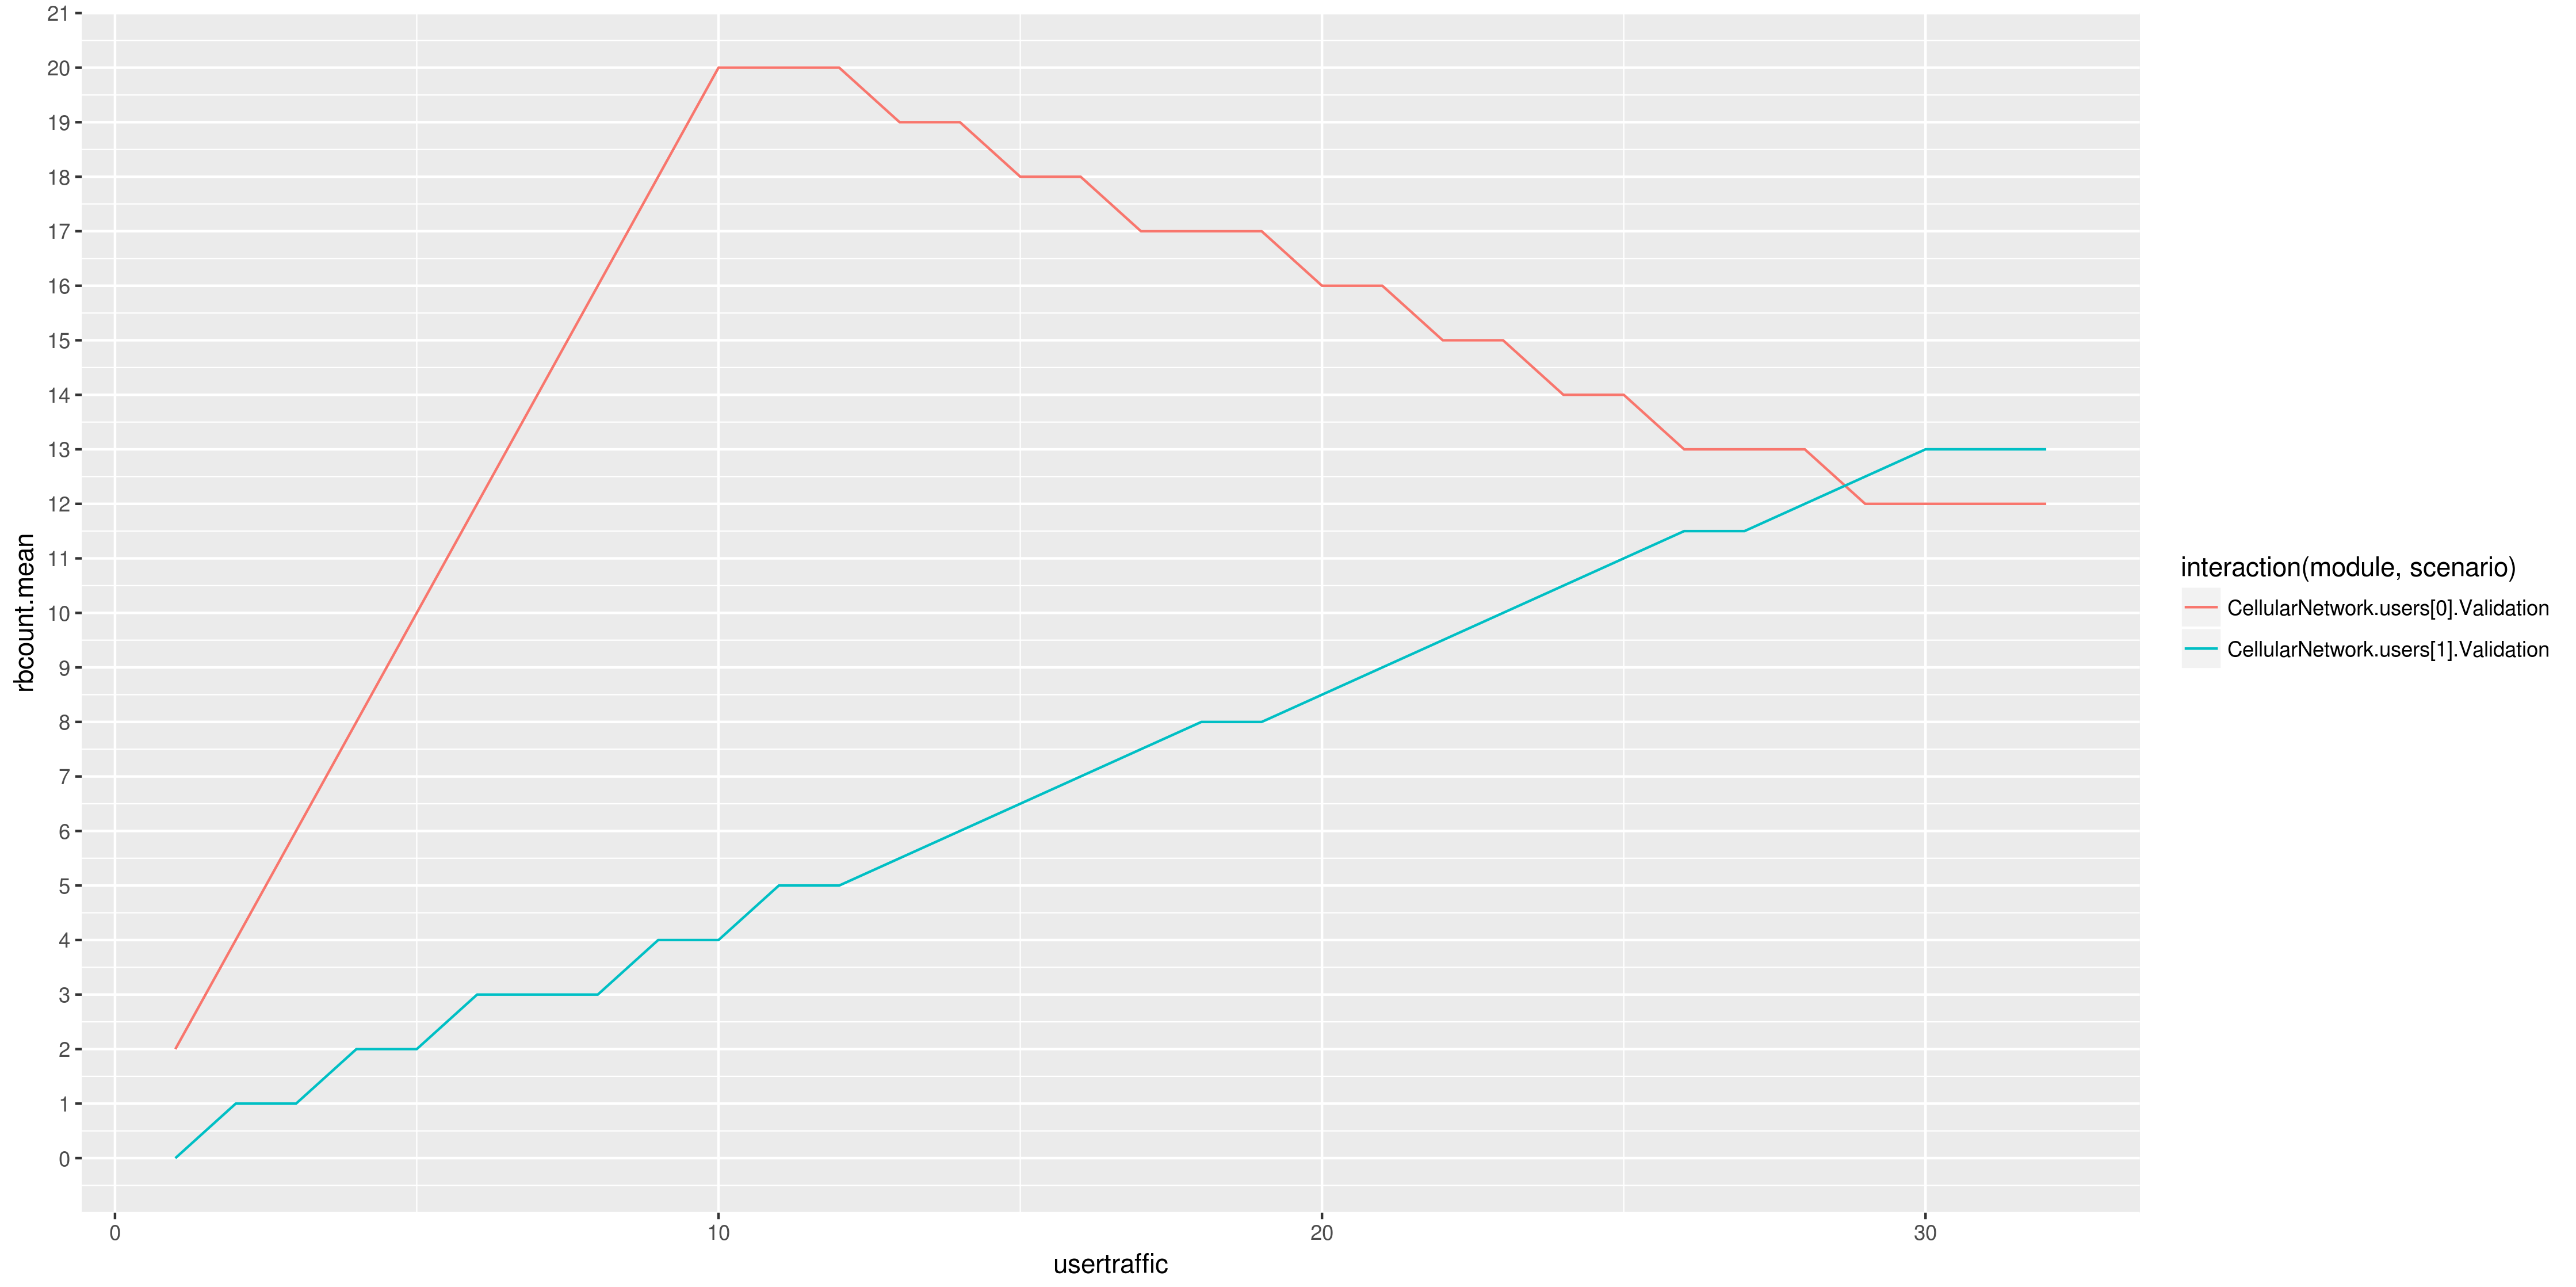
\includegraphics[width=1\textwidth]{images/RBCompvalidation2}
  \caption{2nd validation scenario: mean RB count}
  \label{fig:2nd validation scenario: mean RB count}
\end{figure}
By math the mean RB would be \(\#RB / 2 = 12.5 \) but the number of RB assigned per user is slightly different since, on average, 11 RBs are assigned to \texttt{Mobile User[0]} and 13 RBs are assigned to \texttt{Mobile User[1]}. This oddness is due to fragmentation of packet. In our simple model infact packets could not be fragmented so if a packet does not fill inside the last RB this RB is lost and it assigned to the next user. Note that in validation scenarios everything is fixed, also packet dimension, so there could be strangeness like that. However we can say that our model is quite accurate and can be used to simulate the network in more complex scenarios. 